\documentclass[11pt,a4paper]{article}
\usepackage[T1]{fontenc}
\usepackage[margin=2.3cm]{geometry}
\usepackage{amsmath,amssymb}
\usepackage{graphicx}
\usepackage[dvipsnames]{xcolor}
\usepackage{enumitem}
\usepackage[colorlinks=true,linkcolor=blue,urlcolor=blue]{hyperref}
\setlength{\parskip}{0.6em}
\setlength{\parindent}{0pt}
\begin{document}

\begin{center}{\LARGE\bfseries opendronecontrol}\\[0.4em]{\large Make a quadrotor hover and hold its attitude with PID control, in three sessions.}\\[0.2em]\small PAN IIT OSS explainer \textbullet{} higher secondary to advanced undergraduate (levels 4-6)\end{center}

\section*{Why this exists}
A multicopter hovers by controlling its thrust with feedback, most often with a PID controller. This explainer follows the idea from thrust and weight to a PID altitude hold and a cascaded attitude controller that tilts the drone to move, using only Newton's laws and a few formulas for second-order systems.

\section*{The end goal}
PID hover and attitude control of a quadrotor: to make a drone hold its height when its mass is not known exactly, to tilt it to move sideways and back, and to know from the formulas and the simulation why it is stable, how much it overshoots and what limits the gains. The same ideas run in camera gimbals, self-balancing scooters, cruise control and rocket attitude control.

\section*{How the three sessions build up}
\begin{enumerate}[nosep]
\item \textbf{Session 1: Thrust, weight and hover} (Level 1, conceptual interactive model, 60 min).
\item \textbf{Session 2: Altitude hold with a PID controller} (Level 2, mathematical engineering model, 75 min).
\item \textbf{Session 3: Tilt to move: attitude control and cascaded PID} (Level 3, simulation and validation, 90 min).
\end{enumerate}

\emph{All models here are simplified educational models, not validated design tools. Real drones have sharp spinning propellers; follow your local aviation rules and never test near people.}

\section{Session 1: Thrust, weight and hover}

\subsection*{A. Real-world problem}
A 1.2 kg delivery drone must hover still above a doorstep. Its four rotors push air down and the air pushes the drone up. How fast must the rotors spin to hover? And if someone clips on a 0.2 kg parcel and nobody touches the throttle, what happens in the next two seconds? (General education only: this is a simplified model, not a drone design method. Real drones have sharp spinning propellers; never test near people or without the safety rules of your local aviation authority.)

\subsection*{B. Concept and theory}
Gravity pulls the drone down with its weight W = m g. Each propeller throws air downwards, and by Newton's third law the air pushes the propeller up. For a given propeller in still air the thrust grows with the square of the spin speed: T = k\_T omega\textasciicircum{}2, where omega is in radians per second and k\_T (here 1.0e-5 N per (rad/s)\textasciicircum{}2, typical of a 10-inch propeller) lumps together the propeller's size, shape and the air density. To hover, the n rotors together must carry the weight, so each spins at omega\_hover = sqrt(m g / (n k\_T)). The thrust-to-weight ratio, the largest total thrust divided by the weight, tells you how much spare push is left to climb, fight a gust or correct a tilt; builders aim for at least 2. Taking up as positive, Newton's second law gives m a = T\_total - m g. With the throttle held fixed, a is constant and a drone that starts at rest moves z = a t\textasciicircum{}2 / 2: a small thrust mistake grows into a large height mistake because time is squared. Hovering also costs power even when nothing moves: momentum theory gives an ideal induced power P = T\textasciicircum{}1.5 / sqrt(2 rho A) per rotor of disc area A.

\begin{itemize}[nosep]
\item m: mass of the drone (plus any payload) (kg)
\item g: gravitational acceleration, 9.81 (m/s\textasciicircum{}2)
\item W: weight m g (N)
\item T: thrust of one rotor; T\_total for all rotors (N)
\item omega: rotor spin speed (1 rad/s = 9.549 rpm) (rad/s)
\item k\_T: rotor thrust coefficient (N/(rad/s)\textasciicircum{}2)
\item n: number of rotors (4 for a quadrotor) (no unit)
\item a, z: vertical acceleration and height change, up positive (m/s\textasciicircum{}2, m)
\item rho, A: air density (1.225) and rotor disc area (kg/m\textasciicircum{}3, m\textasciicircum{}2)
\end{itemize}

\begin{equation*}
W = m g,\qquad T = k_T\,\omega^2
\end{equation*}

\begin{equation*}
\omega_{\mathrm{hover}} = \sqrt{\frac{m g}{n\,k_T}},\qquad \text{rpm} = \omega\,\frac{60}{2\pi}
\end{equation*}

\begin{equation*}
\frac{T}{W}\bigg|_{\max} = \frac{n\,k_T\,\omega_{\max}^2}{m g}
\end{equation*}

\begin{equation*}
m\,\ddot z = T_{\mathrm{total}} - m g,\qquad z(t) = \tfrac12 a t^2
\end{equation*}

\begin{equation*}
P_{\mathrm{ideal}} = \frac{T^{3/2}}{\sqrt{2\rho A}}
\end{equation*}

\begin{center}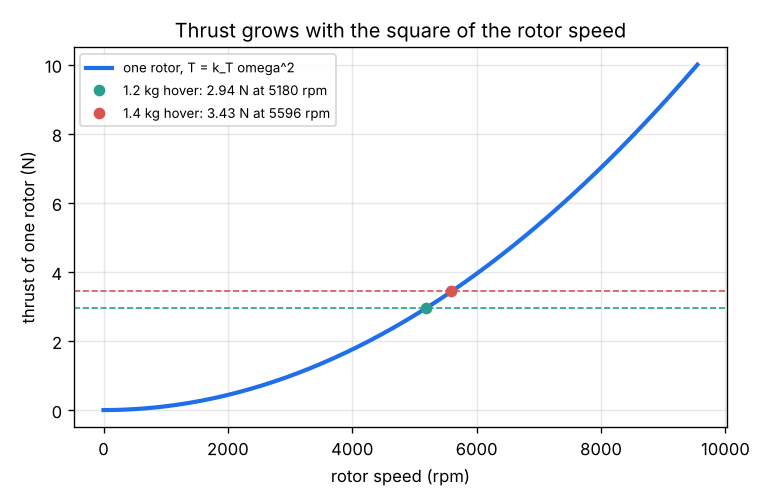
\includegraphics[width=0.85\linewidth]{figures/s01_thrust_curve.png}\\\small Thrust of one rotor against rotor speed, with the hover points of a 1.2 kg and a 1.4 kg drone.\end{center}

\subsection*{E. Worked example}
A 1.2 kg quadrotor has rotors with k\_T = 1.0e-5 N/(rad/s)\textasciicircum{}2 and a top speed of 1000 rad/s. Find its weight, the hover speed in rad/s and rpm, and its thrust-to-weight ratio. Then a 0.2 kg parcel is added with the throttle unchanged: find the acceleration and how long the drone takes to sink 1 m.
\begin{enumerate}[nosep]
\item Weight: W = 1.2 x 9.81 = 11.772 N, so each rotor carries 11.772 / 4 = 2.943 N.
\item Hover speed: omega = sqrt(2.943 / 1.0e-5) = sqrt(294300) = 542.5 rad/s; rpm = 542.5 x 60 / (2 pi) = 5180 rpm.
\item Top thrust: 4 x 1.0e-5 x 1000\textasciicircum{}2 = 40 N, so thrust-to-weight = 40 / 11.772 = 3.40 (enough spare push).
\item With the parcel: m = 1.4 kg, thrust still 11.772 N, so a = 11.772 / 1.4 - 9.81 = 8.409 - 9.81 = -1.40 m/s\textasciicircum{}2 (downwards).
\item Time to sink 1 m: 1 = 0.5 x 1.40 x t\textasciicircum{}2, so t = sqrt(2 / 1.40) = 1.19 s.
\end{enumerate}
\textbf{Answer.} W = 11.77 N, hover at 542.5 rad/s (5180 rpm), thrust-to-weight 3.40; with the parcel the drone accelerates down at 1.40 m/s\textasciicircum{}2 and sinks 1 m in 1.19 s.

\subsection*{F. Questions}
\begin{enumerate}[nosep]
\item \textbf{Conceptual.} A pilot finds the exact throttle at which the drone hovers, then lets go of the stick. Give three reasons why the drone will still drift up or down after a while.
\item \textbf{Numerical.} A smaller 0.9 kg quadrotor uses the same rotors (k\_T = 1.0e-5 N/(rad/s)\textasciicircum{}2, top speed 1000 rad/s). Find the thrust per rotor to hover, the hover speed in rad/s and rpm, and its thrust-to-weight ratio. Check the units and that the answer is reasonable.
\item \textbf{Graph and simulation interpretation.} On the thrust curve, by what factor does the thrust grow when the rotor speed goes from 4000 to 8000 rpm? On the drift graph, the 1.4 kg drone has sunk 2.80 m after 2 s. How far had it sunk after 1 s, and why is that not half?
\item \textbf{Design and optimisation challenge.} Design: you want the 1.2 kg drone to have a thrust-to-weight ratio of at least 2. What top rotor speed (rpm) is needed with k\_T = 1.0e-5? What top speed is needed if it must also carry a 0.4 kg parcel? With the real top speed of 1000 rad/s, what is the largest payload that keeps the ratio at 2?
\end{enumerate}

\section{Session 2: Altitude hold with a PID controller}

\subsection*{A. Real-world problem}
In Session 1 a fixed throttle let the drone sink as soon as a 0.2 kg parcel was added. A flight controller instead measures the height (with a barometer, a downward range sensor or GPS) many times per second and corrects the thrust. How should the correction depend on the error so that the drone climbs to 2 m quickly, without a big overshoot, and ends up exactly at 2 m even though the controller still believes the drone weighs 1.2 kg when it really weighs 1.4 kg? (Simplified one-dimensional model; not a flight-controller design method.)

\subsection*{B. Concept and theory}
Every time step the controller computes the error e = z\_ref - z between the wanted and the measured height. It sets the total thrust T = m\_nom g + u: the first part is a feed-forward guess of the hover thrust using the mass it believes, and u is the feedback correction. A PID controller builds u from three parts: u = Kp e + Ki (integral of e dt) - Kd (dz/dt). The \textbf{P} term pushes back in proportion to the error, like a spring. The \textbf{D} term opposes the climb rate, like a damper or shock absorber; we use the measured rate dz/dt instead of de/dt so that a sudden change of target does not kick the thrust. The \textbf{I} term adds up the error over time and keeps growing while any error remains. Putting T into m z'' = T - m g gives a mass-spring-damper: m z'' + Kd z' + Kp z = Kp z\_ref + (m\_nom - m) g. Its natural frequency is wn = sqrt(Kp / m), its damping ratio is zeta = Kd / (2 sqrt(Kp m)), and for 0 < zeta < 1 a step overshoots by exp(-zeta pi / sqrt(1 - zeta\textasciicircum{}2)) and settles (within 2 percent) in about 4 / (zeta wn). With P alone zeta = 0 and the drone bounces for ever. When the true mass differs from m\_nom, gravity is not fully cancelled and P or PD control settles short by the steady-state error e\_ss = (m - m\_nom) g / Kp. Integral action removes it, but makes the loop third order, m s\textasciicircum{}3 + Kd s\textasciicircum{}2 + Kp s + Ki = 0, which by the Routh test is stable only when Kd Kp > m Ki. Real rotors cannot push down or exceed their maximum, so the thrust is limited to 0 to 40 N.

\begin{itemize}[nosep]
\item z, z\_ref: measured and wanted height (m)
\item e: error z\_ref - z (m)
\item m, m\_nom: true mass, and the mass the controller believes (kg)
\item u: feedback correction to the thrust (N)
\item Kp: proportional gain (N/m)
\item Ki: integral gain (N/(m s))
\item Kd: derivative gain (N s/m)
\item wn: natural frequency (rad/s)
\item zeta: damping ratio (no unit)
\item e\_ss: steady-state error (m)
\end{itemize}

\begin{equation*}
e = z_{\mathrm{ref}} - z,\qquad T = m_{\mathrm{nom}}\,g + K_p e + K_i\!\int e\,dt - K_d\,\dot z
\end{equation*}

\begin{equation*}
\omega_n = \sqrt{\frac{K_p}{m}},\qquad \zeta = \frac{K_d}{2\sqrt{K_p m}}
\end{equation*}

\begin{equation*}
M_p = \exp\!\left(\frac{-\zeta\pi}{\sqrt{1-\zeta^2}}\right),\qquad t_s \approx \frac{4}{\zeta\,\omega_n}
\end{equation*}

\begin{equation*}
e_{ss} = \frac{(m - m_{\mathrm{nom}})\,g}{K_p}\quad(\text{P or PD}),\qquad e_{ss} = 0\quad(\text{PID})
\end{equation*}

\begin{equation*}
m s^3 + K_d s^2 + K_p s + K_i = 0\ \text{stable} \iff K_d K_p > m K_i
\end{equation*}

\begin{center}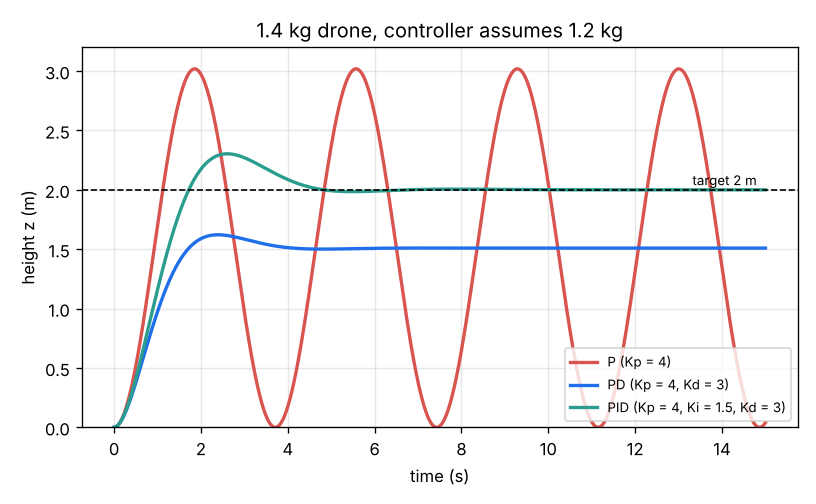
\includegraphics[width=0.85\linewidth]{figures/s02_p_pd_pid.png}\\\small P, PD and PID control of a 1.4 kg drone whose controller assumes 1.2 kg.\end{center}

\subsection*{E. Worked example}
A PD altitude controller with Kp = 4 N/m and Kd = 3 N s/m believes the drone weighs 1.2 kg, but it really weighs 1.4 kg. Find wn, zeta, the overshoot and the settling time of a climb to 2 m, and the final height. Then add Ki = 1.5 N/(m s) and check it is stable.
\begin{enumerate}[nosep]
\item Natural frequency: wn = sqrt(4 / 1.4) = sqrt(2.857) = 1.690 rad/s.
\item Damping ratio: zeta = 3 / (2 sqrt(4 x 1.4)) = 3 / (2 x 2.366) = 0.634.
\item Overshoot: sqrt(1 - 0.634\textasciicircum{}2) = 0.773; exp(-0.634 x 3.1416 / 0.773) = exp(-2.576) = 0.076, so 7.6 percent. Settling time about 4 / (0.634 x 1.690) = 3.7 s.
\item Steady-state error: (1.4 - 1.2) x 9.81 / 4 = 1.962 / 4 = 0.4905 m, so the drone settles at 2 - 0.49 = 1.51 m.
\item With Ki = 1.5: Kd Kp = 12 is larger than m Ki = 2.1, so the PID loop is stable and the error goes to zero; at rest the thrust is the true weight 1.4 x 9.81 = 13.73 N.
\end{enumerate}
\textbf{Answer.} wn = 1.69 rad/s, zeta = 0.63, overshoot 7.6 percent, settling about 3.7 s, PD settles at 1.51 m (0.49 m short). The simulation gives 7.4 percent, 3.5 s and 1.509 m. PID is stable and settles at 2.000 m.

\subsection*{F. Questions}
\begin{enumerate}[nosep]
\item \textbf{Conceptual.} Why does a PD controller leave the heavier drone below its target, and how does adding the I term fix it? What does the I term cost?
\item \textbf{Numerical.} For the 1.4 kg drone choose Kp = 8 N/m. What Kd gives zeta = 0.7? Find wn, the overshoot, the settling time and the PD steady-state error. Check that the answers are reasonable compared with the worked example.
\item \textbf{Graph and simulation interpretation.} In Figure 2 (left), Kd = 0.8, 1.5, 3 and 6 N s/m. Predict the overshoot of each from the formula and say which curve has none. Why is the Kd = 6 curve the slowest to rise even though it has the most "control"?
\item \textbf{Design and optimisation challenge.} Design: the drone (1.4 kg, controller believes 1.2 kg) must reach 2 m with overshoot below 10 percent, settle within 4 s, and end within 2 cm of the target. The thrust is limited to 40 N. Choose Kp, Ki and Kd and justify them. What is the largest Ki the Routh test allows for your Kp and Kd?
\end{enumerate}

\section{Session 3: Tilt to move: attitude control and cascaded PID}

\subsection*{A. Real-world problem}
A drone has no sideways propeller. To move 1 m to the right it must lean right so part of its thrust points sideways, and then lean left to stop. It leans by spinning the rotors on one side faster than on the other. The rotors cannot change speed instantly, and while the drone leans, less thrust points up. How do we build a controller that flies a camera drone 1 m sideways in a few seconds, keeps its height, never tilts more than the camera can cope with, and stays stable with real, slow motors? (A simplified teaching model, not a flight-controller design tool.)

\subsection*{B. Concept and theory}
Look at the drone from behind: it has a sideways position y, a height z and a roll angle phi (positive = leaning right). The left and right rotor pairs give forces F\_l and F\_r. Their sum is the thrust T along the drone's own "up" axis; their difference, times the arm length L, is the roll torque tau = (F\_l - F\_r) L. Newton's laws give m y'' = T sin(phi), m z'' = T cos(phi) - m g and I phi'' = tau, where I is the moment of inertia: the rotational version of mass, which measures how hard the drone is to spin. A \textbf{mixer} inverts this: F\_l = T / 2 + tau / (2L), F\_r = T / 2 - tau / (2L). The controller is a \textbf{cascade} of loops. The outer position loop asks for an acceleration a\_y = Kp\_y (y\_ref - y) - Kd\_y vy, and since y'' is about g phi for small angles it asks the inner loop for a tilt phi\_des = a\_y / g, limited to 30 degrees. The inner attitude loop is a PD: tau = Kp\_att (phi\_des - phi) - Kd\_att p, with p the roll rate. Since I phi'' = tau is the same "push a mass" problem as Session 2, it has wn\_att = sqrt(Kp\_att / I) and zeta\_att = Kd\_att / (2 sqrt(Kp\_att I)). The height loop is Session 2's PID; dividing its thrust by cos(phi) (\textbf{tilt compensation}) keeps the vertical part of the thrust right while leaning. A rule of thumb is to make the inner loop 5 to 10 times faster than the outer loop, so the outer loop can treat the tilt as instant. Real motors lag: a first-order model dF/dt = (F\_cmd - F) / tau\_m makes the attitude loop third order, I tau\_m s\textasciicircum{}3 + I s\textasciicircum{}2 + Kd\_att s + Kp\_att = 0, and the Routh test gives the stability limit tau\_m < Kd\_att / Kp\_att. A stiffer attitude loop therefore needs faster motors.

\begin{itemize}[nosep]
\item y, z: sideways position and height change (m)
\item phi, p: roll angle and roll rate (rad (degrees in plots), rad/s)
\item F\_l, F\_r: forces of the left and right rotor pairs (N)
\item T, tau: total thrust and roll torque (N, N m)
\item L: arm from the centre to each rotor pair, 0.2 (m)
\item I: roll moment of inertia, 0.012 (kg m\textasciicircum{}2)
\item Kp\_att, Kd\_att: attitude gains (N m/rad, N m s/rad)
\item Kp\_y, Kd\_y: position gains (per unit mass) (1/s\textasciicircum{}2, 1/s)
\item tau\_m: motor time constant (s)
\end{itemize}

\begin{equation*}
m\ddot y = T\sin\phi,\qquad m\ddot z = T\cos\phi - m g,\qquad I\ddot\phi = (F_l - F_r)L
\end{equation*}

\begin{equation*}
F_{l,r} = \frac{T}{2} \pm \frac{\tau}{2L},\qquad T = \frac{m(g + a_z)}{\cos\phi}
\end{equation*}

\begin{equation*}
\phi_{\mathrm{des}} = \frac{K_{p,y}(y_{\mathrm{ref}} - y) - K_{d,y}\dot y}{g},\qquad \tau = K_{p,\mathrm{att}}(\phi_{\mathrm{des}} - \phi) - K_{d,\mathrm{att}}\,\dot\phi
\end{equation*}

\begin{equation*}
\omega_{n,\mathrm{att}} = \sqrt{\frac{K_{p,\mathrm{att}}}{I}},\qquad \zeta_{\mathrm{att}} = \frac{K_{d,\mathrm{att}}}{2\sqrt{K_{p,\mathrm{att}} I}}
\end{equation*}

\begin{equation*}
\tau_m\frac{dF}{dt} = F_{\mathrm{cmd}} - F,\qquad \text{stable} \iff \tau_m < \frac{K_{d,\mathrm{att}}}{K_{p,\mathrm{att}}}
\end{equation*}

\begin{center}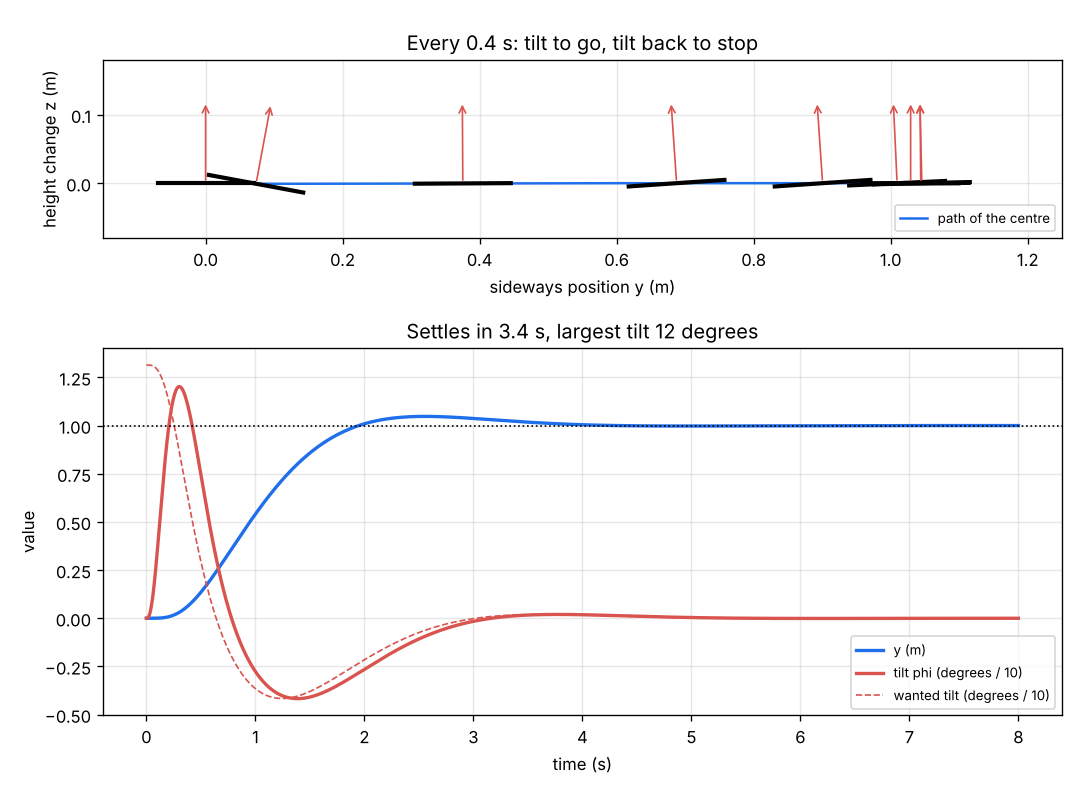
\includegraphics[width=0.85\linewidth]{figures/s03_sideways_move.png}\\\small A 1 m sideways move: the drone leans to go, leans back to stop, and ends level at y = 1 m.\end{center}

\subsection*{E. Worked example}
The drone (m = 1.2 kg, I = 0.012 kg m\textasciicircum{}2, L = 0.2 m) uses Kp\_att = 1.2 N m/rad and Kd\_att = 0.17 N m s/rad. Find the attitude wn, zeta and overshoot, and the motor-lag limit. At the start of a 1 m move with Kp\_y = 2.25 1/s\textasciicircum{}2, find the tilt the outer loop asks for, the first roll torque and the two rotor forces.
\begin{enumerate}[nosep]
\item Attitude loop: wn = sqrt(1.2 / 0.012) = sqrt(100) = 10 rad/s; zeta = 0.17 / (2 sqrt(1.2 x 0.012)) = 0.17 / (2 x 0.12) = 0.708.
\item Overshoot = exp(-0.708 pi / sqrt(1 - 0.708\textasciicircum{}2)) = exp(-0.708 x 3.1416 / 0.706) = exp(-3.15) = 0.043, so 4.3 percent.
\item Motor-lag limit: tau\_m < 0.17 / 1.2 = 0.142 s. Motors with 0.02 s or 0.06 s are fine; 0.15 s would make the drone shake.
\item Wanted tilt at the start: phi\_des = 2.25 x (1 - 0) / 9.81 = 0.229 rad = 13.1 degrees.
\item First torque: tau = 1.2 x 0.229 = 0.275 N m. With T = 11.772 N: F\_l = 5.886 + 0.275 / 0.4 = 6.574 N and F\_r = 5.886 - 0.688 = 5.198 N. The left rotors push harder, so the drone rolls right.
\end{enumerate}
\textbf{Answer.} wn = 10 rad/s, zeta = 0.71, overshoot 4.3 percent (simulated 4.2 percent), lag limit 0.142 s; the drone asks for 13.1 degrees and commands 6.57 N left and 5.20 N right. The full simulation settles at y = 1.000 m in 3.4 s with a 5 cm overshoot and a largest tilt of 12 degrees.

\subsection*{F. Questions}
\begin{enumerate}[nosep]
\item \textbf{Conceptual.} Why must the inner attitude loop be much faster than the outer position loop? What happens if it is too slow, and what happens if you make it very fast?
\item \textbf{Numerical.} For candidate B (Kp\_att = 0.432 N m/rad, Kd\_att = 0.1008 N m s/rad, I = 0.012 kg m\textasciicircum{}2) find wn, zeta, the overshoot and the motor-lag limit. Is it safe with 0.06 s motors and a safety factor of 2? With 0.10 s motors?
\item \textbf{Graph and simulation interpretation.} In Figure 2 (left), describe how the tilt response changes as tau\_m goes from 0 to 0.13 s. Why does the motor lag make the tilt overshoot more, even though the gains did not change?
\item \textbf{Design and optimisation challenge.} Design: the motors are replaced by cheaper ones with tau\_m = 0.10 s. Choose Kp\_att and Kd\_att so that the 1 m move settles within 4 s, the tilt stays at or below 15 degrees, and the lag limit has a safety factor of 2. Justify your choice and state the trade-off.
\end{enumerate}

\section{Real-world mini-project}
\textbf{Tune the attitude loop of a camera drone.} A camera drone (the Session 3 model) must move 1 m sideways and settle within 4 s, dip less than 1 cm, and never tilt more than 15 degrees so its camera gimbal can cope. Its motors have a time constant of 0.06 s, and the designer wants a safety factor of 2 on the lag limit: tau\_m must be at most Kd\_att / (2 Kp\_att). Four candidate attitude tunings are offered, all with zeta = 0.7: A soft (wn = 4 rad/s: Kp\_att = 0.192, Kd\_att = 0.0672), B medium (wn = 6: 0.432, 0.1008), C default (wn = 10: 1.2, 0.17) and D stiff (wn = 20: 4.8, 0.336). Use \texttt{check\_design} from Session 3. These limits are illustrative, not a product specification.

\section{The path ahead}
\begin{enumerate}[nosep]
\item \textbf{Session 4: The rate loop and gyroscope noise.} A rate loop (PI on the roll rate) inside the Session 3 attitude loop, gyro readings with 0.05 rad/s of random noise, and a low-pass filter on the derivative.
\item \textbf{Session 5: Integrator wind-up and wind gusts.} Anti-wind-up for the height PID and a side-wind force on the planar drone, with an I term in the position loop.
\item \textbf{Session 6: The full 3-D quadrotor.} A 12-state rigid-body model with four motors and the cascaded PID on all three axes.
\item \textbf{Session 7: Estimating the state.} Simulated gyro (with bias) and accelerometer readings and a complementary filter; the controller flies on the estimate, not on the true state.
\item \textbf{Session 8: Fly a square mission.} Take-off to 1.5 m, a 2 m square, landing, and a gust halfway, flown by the 3-D model of Session 6 with the estimator of Session 7.
\end{enumerate}

\section{Answers and hints}

\subsection*{Session 1}
\begin{enumerate}[nosep]
\item \textbf{Conceptual.} Hint: What in m a = T - m g, or in T = k\_T omega\textasciicircum{}2, could change during the flight without the throttle moving? Solution: Any change that breaks T = m g makes a nonzero acceleration, and the height error then grows like t squared. Examples: (1) the battery voltage falls as it drains, so the motors spin slower at the same throttle and thrust drops; (2) the mass changes (a parcel, rain, a camera); (3) the air changes: a warmer day or a higher place has lower density, which lowers k\_T, and gusts or ground effect change the thrust. Since we never know these exactly, the throttle must be corrected all the time from a measurement: feedback.
\item \textbf{Numerical.} Hint: T per rotor = m g / 4, then omega = sqrt(T / k\_T), then rpm = omega x 60 / (2 pi). Solution: T = 0.9 x 9.81 / 4 = 2.207 N per rotor. omega = sqrt(2.207 / 1.0e-5) = sqrt(220700) = 469.8 rad/s = 4486 rpm. Thrust-to-weight = 40 / 8.829 = 4.53. Sanity check: the lighter drone hovers at a lower speed than the 1.2 kg one (5180 rpm), and the ratio of speeds 4486 / 5180 = 0.866 equals sqrt(0.9 / 1.2) = 0.866, as the square-root law says.
\item \textbf{Graph and simulation interpretation.} Hint: T is proportional to omega\textasciicircum{}2, and z is proportional to t\textasciicircum{}2. Solution: Doubling the speed multiplies the thrust by 2\textasciicircum{}2 = 4. For the drift, z = a t\textasciicircum{}2 / 2, so halving the time divides the drop by 4: 2.80 / 4 = 0.70 m after 1 s. It is not half because the drone keeps speeding up: its downward speed grows steadily, so each second it falls further than in the second before.
\item \textbf{Design and optimisation challenge.} Hint: Ratio 2 means each rotor must reach 2 m g / 4. The largest total thrust at 1000 rad/s is 40 N. Solution: Empty: each rotor needs 2 x 11.772 / 4 = 5.886 N, so omega = sqrt(588600) = 767.2 rad/s = 7326 rpm. With 0.4 kg: m = 1.6 kg, each rotor needs 2 x 15.696 / 4 = 7.848 N, omega = 885.9 rad/s = 8460 rpm. At 1000 rad/s the total is 40 N, so the weight may be at most 20 N, m at most 2.04 kg and the payload at most 0.84 kg. Trade-off: more payload means less spare thrust for climbing and correcting, and much more power (it grows as mass\textasciicircum{}1.5).
\end{enumerate}

\subsection*{Session 2}
\begin{enumerate}[nosep]
\item \textbf{Conceptual.} Hint: At rest z' = 0, so the D term is zero. What must the P term supply on its own? Solution: At rest the drone must make thrust equal to its true weight. The feed-forward supplies m\_nom g, which is 1.96 N too little. With z' = 0 the D term is zero, so the P term must supply the missing 1.96 N, and it can only do that if an error remains: Kp e = 1.96 N, so e = 0.49 m. The I term keeps adding up the error, so it keeps growing until it supplies the 1.96 N by itself; then the error can be zero. The cost: the integral builds up during the climb and makes the drone overshoot more (15 percent instead of 7 percent), and too much Ki (above Kd Kp / m) makes the loop unstable.
\item \textbf{Numerical.} Hint: Kd = 2 zeta sqrt(Kp m); then use the formulas of Section B. Solution: sqrt(8 x 1.4) = 3.347, so Kd = 2 x 0.7 x 3.347 = 4.69 N s/m. wn = sqrt(8 / 1.4) = 2.390 rad/s. Overshoot = exp(-0.7 pi / 0.714) = 0.046, so 4.6 percent. Settling about 4 / (0.7 x 2.390) = 2.4 s. Steady-state error 1.962 / 8 = 0.245 m. Reasonable: doubling Kp halved the error and made the drone faster, and the extra Kd kept the overshoot small. The simulation gives 4.3 percent, 2.5 s and 1.755 m.
\item \textbf{Graph and simulation interpretation.} Hint: zeta = Kd / (2 sqrt(4 x 1.4)) = Kd / 4.733. Solution: zeta = 0.17, 0.32, 0.63 and 1.27, so overshoot = 58, 35, 7.6 and 0 percent. Kd = 6 is overdamped (zeta above 1): no overshoot. It rises slowest because the D term opposes any climb rate: a strong damper brakes the drone even while it is still far below the target. Good tuning usually sits near zeta = 0.6 to 0.8, a balance between overshoot and speed.
\item \textbf{Design and optimisation challenge.} Hint: Start from a PD with zeta near 0.7 and wn near 3 rad/s, then add a small Ki and check Kd Kp > m Ki. Use the app's challenge. Solution: One good design: Kp = 12 N/m gives wn = sqrt(12 / 1.4) = 2.93 rad/s; Kd = 5.7 N s/m gives zeta = 5.7 / (2 sqrt(16.8)) = 0.695 (about 5 percent overshoot as a PD). Add Ki = 2 N/(m s) to remove the 0.16 m PD error. Routh: Ki must stay below Kd Kp / m = 68.4 / 1.4 = 48.9, so Ki = 2 is far from the limit. The simulation gives 4.6 percent overshoot, settling in 2.1 s, final height 2.000 m, and a peak thrust of 35.8 N, inside the 40 N limit. Trade-off: larger Kp is faster but asks for more thrust at the start; with Kp much above 12 the thrust saturates and the formulas no longer hold.
\end{enumerate}

\subsection*{Session 3}
\begin{enumerate}[nosep]
\item \textbf{Conceptual.} Hint: The outer loop assumes the tilt it asks for appears at once. Look at candidates A and D in the mini-project. Solution: The outer loop computes the tilt it needs as if the drone tilted instantly. If the inner loop is slow (candidate A, wn = 4 rad/s against the outer 1.5 rad/s), the real tilt lags the wanted tilt, the drone keeps accelerating too long, overshoots and swings back and forth (it settles in 7.1 s). If the inner loop is very fast (candidate D, wn = 20 rad/s), it needs a big Kp\_att; then the motor lag matters: the limit Kd/Kp falls to 0.070 s, close to the real 0.06 s, and the tilt overshoots to 18.5 degrees. So the inner loop should be faster than the outer loop by about 5 to 10 times, but no faster than the motors allow.
\item \textbf{Numerical.} Hint: wn = sqrt(Kp / I), zeta = Kd / (2 sqrt(Kp I)), limit = Kd / Kp. Solution: wn = sqrt(0.432 / 0.012) = sqrt(36) = 6 rad/s. sqrt(0.432 x 0.012) = 0.072, so zeta = 0.1008 / 0.144 = 0.70. Overshoot = exp(-0.7 pi / 0.714) = 0.046, 4.6 percent. Limit = 0.1008 / 0.432 = 0.233 s. With 0.06 s motors: 2 x 0.06 = 0.12 s is below 0.233 s, safe. With 0.10 s motors: 0.20 s is still below 0.233 s, safe. (Candidate C, limit 0.142 s, would fail the safety factor with 0.10 s motors.)
\item \textbf{Graph and simulation interpretation.} Hint: When the controller asks the right rotors to slow down, when does the force actually change? Solution: At tau\_m = 0 the tilt rises smoothly with a small 4 percent overshoot. At 0.03 s it is almost the same; at 0.08 s it overshoots to about 6.4 degrees and rings; at 0.13 s it swings to about 7.5 degrees and keeps oscillating for a long time. The lag means the braking torque that the D term asks for arrives late, so the drone is still rotating when it passes the target. The effect is like a delay added to the loop; when the lag reaches Kd/Kp = 0.142 s the oscillation no longer dies out.
\item \textbf{Design and optimisation challenge.} Hint: The safety factor needs Kd / Kp at least 0.20 s. Try the app's challenge with tau\_m = 0.10 s. Solution: Kd / Kp must be at least 2 x 0.10 = 0.20 s, which rules out the default (0.142 s). Candidate B (0.432, 0.1008; limit 0.233 s) meets the margin; one slider-friendly choice in the app is Kp\_att = 0.4 and Kd\_att = 0.10 (limit 0.25 s, wn = 5.8 rad/s, zeta = 0.72). The simulation then settles in about 2.9 s with a largest tilt of about 13.5 degrees and a dip of about 0.5 cm. Trade-off: a softer attitude loop is more tolerant of slow motors, but if it is made too soft (below about wn = 4 rad/s) the outer loop outruns it and the move gets slower and swings. All numbers come from the simplified planar model.
\end{enumerate}

\section{How to join}
Read \texttt{CONTRIBUTING.md} in the repository, then pick an issue labelled \texttt{good first issue}. Repository: \url{https://github.com/KrunalPanchal1995/pan-iit-oss/tree/main/opendronecontrol}

\end{document}
